\section{Systematic uncertainties}\label{sec:systematics}
In this analysis, the systematic uncertainties of the quantities described in Section \ref{sec:methodology} can be divided into three main categories: 
\begin{description}
\item[Neutrino generator.] Our Monte Carlo simulation relies on the neutrino generator provided by the GENIE collaboration \cite{genie}. This generator can be configured to use different physics models, which can affect the relative abundance and the energy of the particles in the final state.
\item[Flux simulation.] The amount of $\nu_{\mu}$ and $\nu_{e}$ reaching the MicroBooNE detector is evaluated by an independent simulation of the neutrino flux of the BNB, used also in the MiniBooNE experiment. This simulation is affected by some uncertainties that need to be taken into account.
\item[Detector simulation.] The detector response (noise removal, signal processing, hit reconstruction) must be carefully simulated in order to achieve a good agreement between data and Monte Carlo in the reconstructed quantities used for background rejection. 
\end{description}

The systematic uncertainties related to the neutrino generator and the flux are evaluated by simulating several \emph{universes}, where the GENIE and flux parameters are varied within their uncertainties. The covariance matrix is defined as:
\begin{equation}
    E_{ij}^{\mathrm{flux, GENIE}} = \frac{1}{N_{u}} \sum^{N_{u}}_{u=0} (x^{u}_{i} - x^{cv}_{i}) (x^{u}_{j} - x^{cv}_{j}),\label{eq:covariance}
\end{equation}
where $i,j$ are the bins of the $x$ reconstructed variable, $N_{u}$ is the number of simulated universes (100 in our case), $x^{u}$ is the reconstructed variable in the $u$ universe and $x^{cv}$ is the central value of the reconstructed variable. 
The detector systematic uncertainties are instead evaluated by varying one parameter per time. In this case, the covariance matrix is:
\begin{equation}
    E_{ij}^{\mathrm{det}} = \sum^{v}_{s=0} (x^{s}_{i} - x^{cv}_{i}) (x^{s}_{j} - x^{cv}_{j}),\label{eq:cov_det}
\end{equation}
where $v$ is the number of detector variations samples and $x^{s}$ is the value of the reconstructed variable in the $s$ sample. The total covariance matrix $E$ is defined as:
\begin{equation}
    E = E^{\mathrm{stat}} + E^{\mathrm{GENIE}} + E^{\mathrm{flux}} + E^{\mathrm{det}},\label{eq:cov_tot}
\end{equation}
where $E^{\mathrm{stat}}$ corresponds to the statistical uncertainty of the Monte Carlo and data off-beam samples, given their limited size. 
The systematic uncertainty for the bin $i$, shown in the plots of Section \ref{sec:methodology}, corresponds to $\sqrt{E_{ii}}$. The fractional covariance matrix $F$ is directly obtained from the covariance matrix and the central values as:
\begin{equation} 
    F_{ij} = \frac{E_{ij}}{x_{i}^{cv} x_{j}^{cv}}.
\end{equation}

\subsection{GENIE systematic uncertainties}
In order to estimate the GENIE systematic uncertainties, the standard GENIE parameters described in \cite{genie} are simultaneously varied within their uncertainties in $N_{u} = 100$ simulated universes. To each universe it will correspond a \emph{weight}, which is applied when filling the histograms of the reconstructed quantities.

Figure \ref{fig:eff_genie} shows the central value of the $\nu_{e}$ CC0$\pi$-Np selection efficiency and the corresponding value for each GENIE variation universe. The variation in this case is expected to be small, since we are essentially dividing two distributions with the same weight. Figure \ref{fig:reco_genie} and Figure \ref{fig:frac_genie} show that the variations in the reconstructed energy spectrum are larger at lower energies, which is the energy region most affected by the GENIE parameters' uncertainties. The GENIE-related uncertainty in the number of selected events from the BNB+cosmic sample is 7.6\%.


\begin{figure}[htbp]
  \begin{center}
    \begin{subfigure}{0.45\textwidth}
      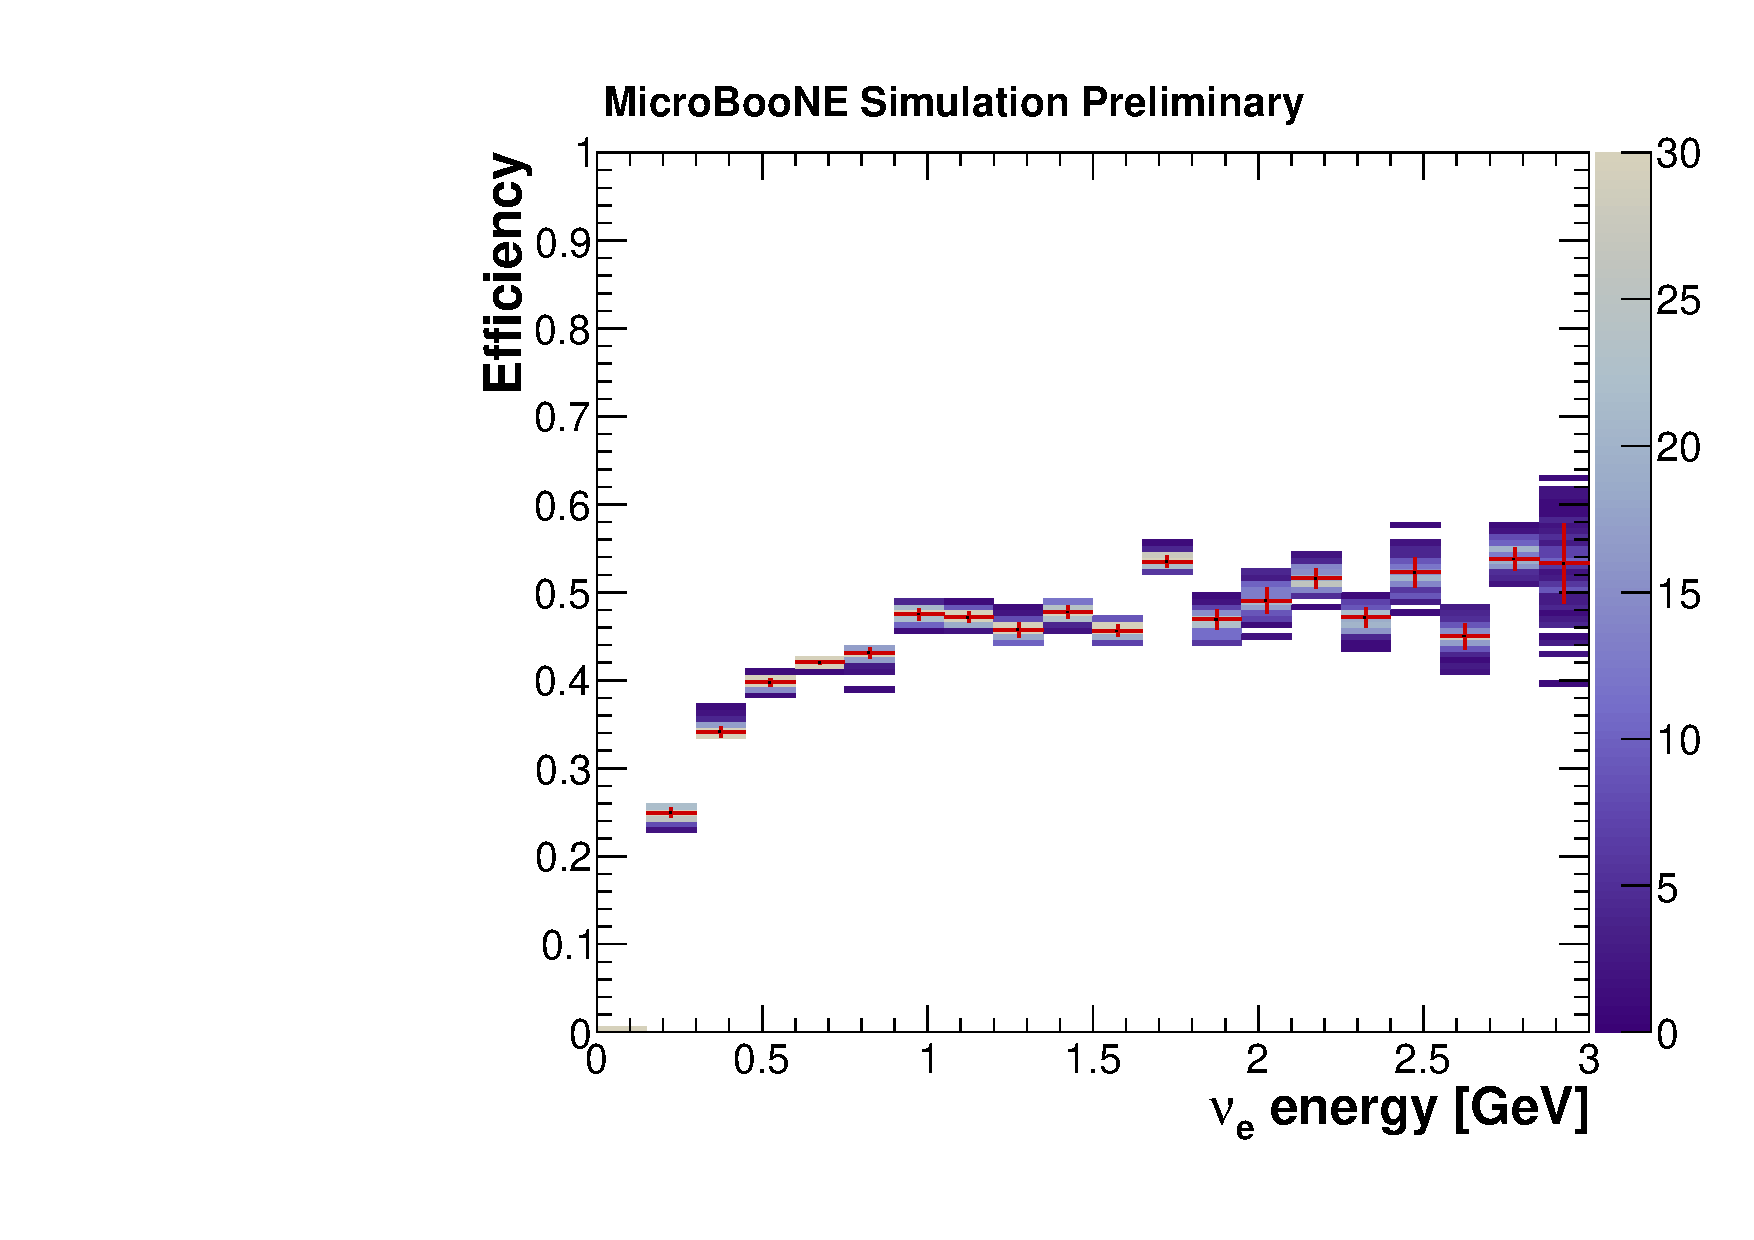
\includegraphics[width=\linewidth]{figures/eff_ene_genie.pdf}
      \caption{$\nu_{e}$ CC0$\pi$-Np selection efficiency.}  \label{fig:eff_genie}
    \end{subfigure}
    \begin{subfigure}{0.45\textwidth}
      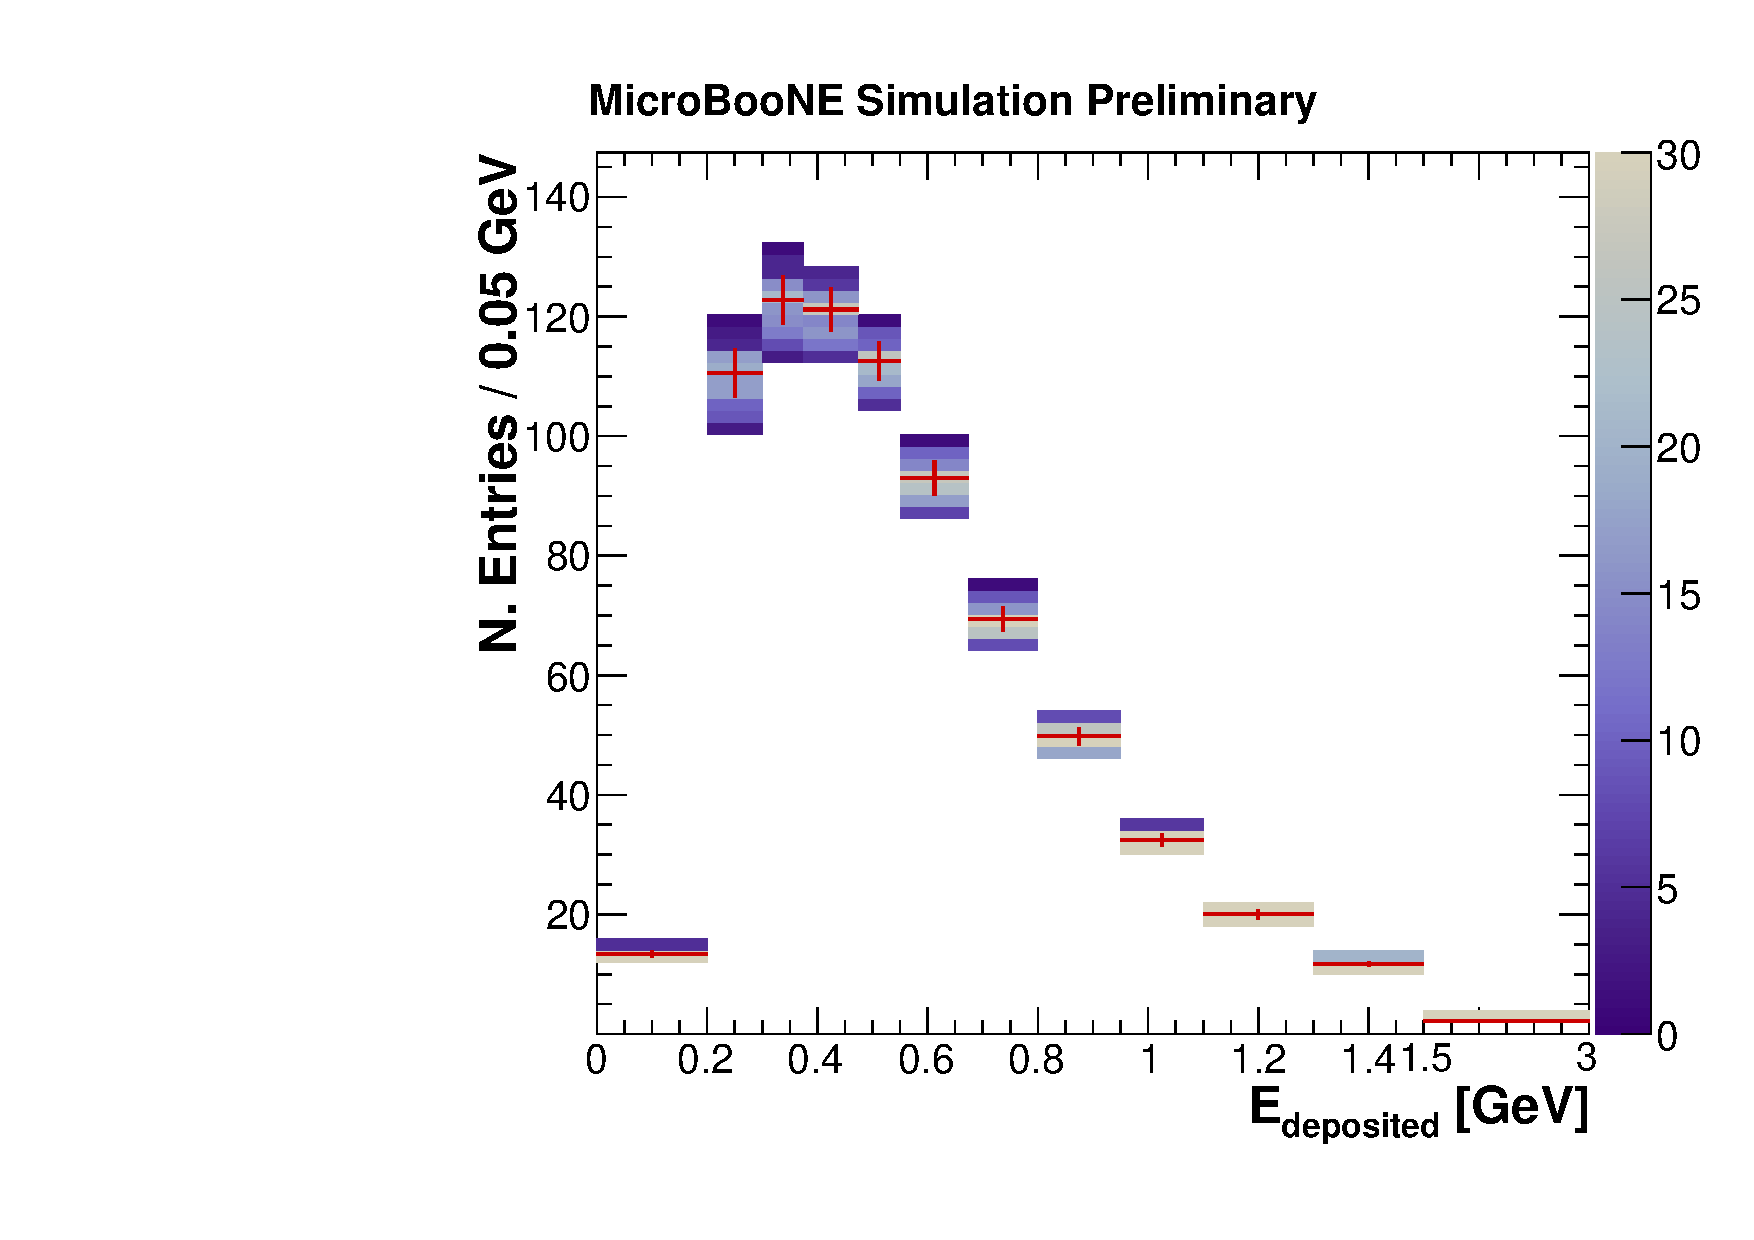
\includegraphics[width=\linewidth]{figures/reco_genie.pdf}
      \caption{$\nu_{e}$ CC0$\pi$-Np candidates energy spectrum in the BNB+cosmic sample.}  \label{fig:reco_genie}
    \end{subfigure}
    \begin{subfigure}{0.45\textwidth}
      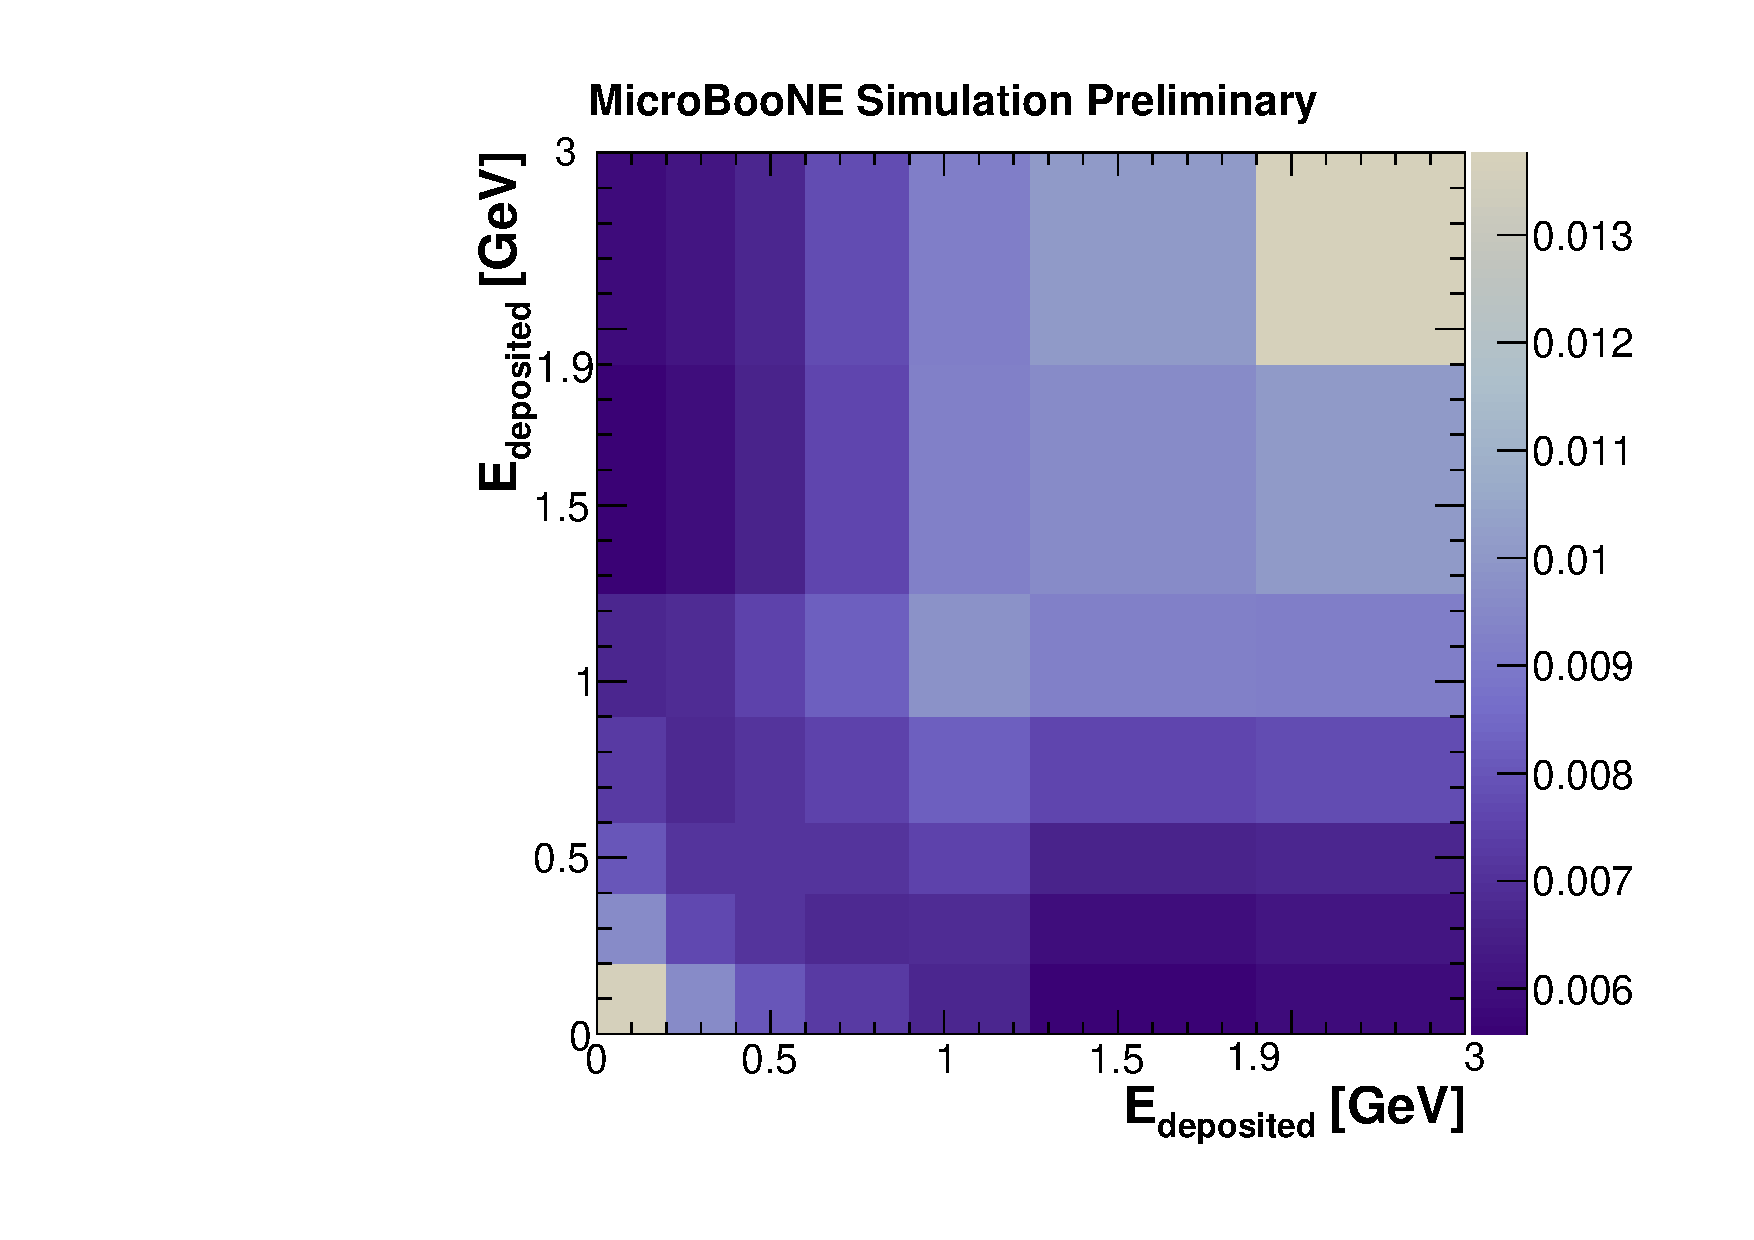
\includegraphics[width=\linewidth]{figures/frac_genie.pdf}
      \caption{GENIE variations fractional covariance matrix.}  \label{fig:frac_genie}
    \end{subfigure}
    	\caption{Selection efficiency, reconstructed energy spectrum, and fractional covariance matrix obtained by varying the standard GENIE parameters in 100 simulated universes. The red bars correspond to the central value and its GENIE systematic uncertainty only.} \label{fig:genie_sys}
	\end{center}
\end{figure}


\subsection{Flux systematic uncertainties}
MicroBooNE is using the same simulation of the BNB flux of the MiniBooNE collaboration. The systematic uncertainties of this simulation, thoroughly described in \cite{miniboone_flux}, can be divided into five main categories:
\begin{description}
\item[Proton delivery:] the numbers of protons hitting the target is affected by the uncertainties in the proton beam optics, which in turns affects the amount of neutrinos in the beam.
\item[Particle production]. The rate and spectrum of secondary particles in the interaction between the protons and the beryllium (the target material) affects the rate and spectrum of the neutrinos. This is main uncertainty in the flux simulation \cite{miniboone_flux}.
\item[Hadronic interactions:] the rate and shape of the flux is affected by the rate of hadronic interactions and the hadronic survival probability both in the target and in the horn.
\item[Horn magnetic field:] uncertainties in the distribution of the magnetic field affect the spectrum of the neutrino flux.
\item[Beamline geometry:] misalignments or displacements of the beamline with respect to the detector can affect the relative neutrino flavour abundances and the flux rate.
\end{description}

In this analysis, the systematic uncertainties related to the flux simulation are evaluated by generating 100 universes, where the flux parameters are varied within their uncertainties. 

Figure \ref{fig:eff_flux} shows the central value of the $\nu_{e}$ CC0$\pi$-Np selection efficiency and the corresponding value for each flux variation universe. Also here, the variation in the efficiency is small, as expected. Figure \ref{fig:reco_flux} shows a bias of the variation samples with respect to the nominal simulation, which does not correspond to the average of the universes. This is caused by an inconsistency of the pion production cross-section used in the generation of the universes \cite{ubxsec, harp}. In this case, the nominal value is considered as the central value in the covariance matrix definition \eqref{eq:covariance}. The flux-related uncertainty in the number of selected events from the BNB+cosmic sample is 7.8\%.

\begin{figure}[htbp]
  \begin{center}
    \begin{subfigure}{0.45\textwidth}
      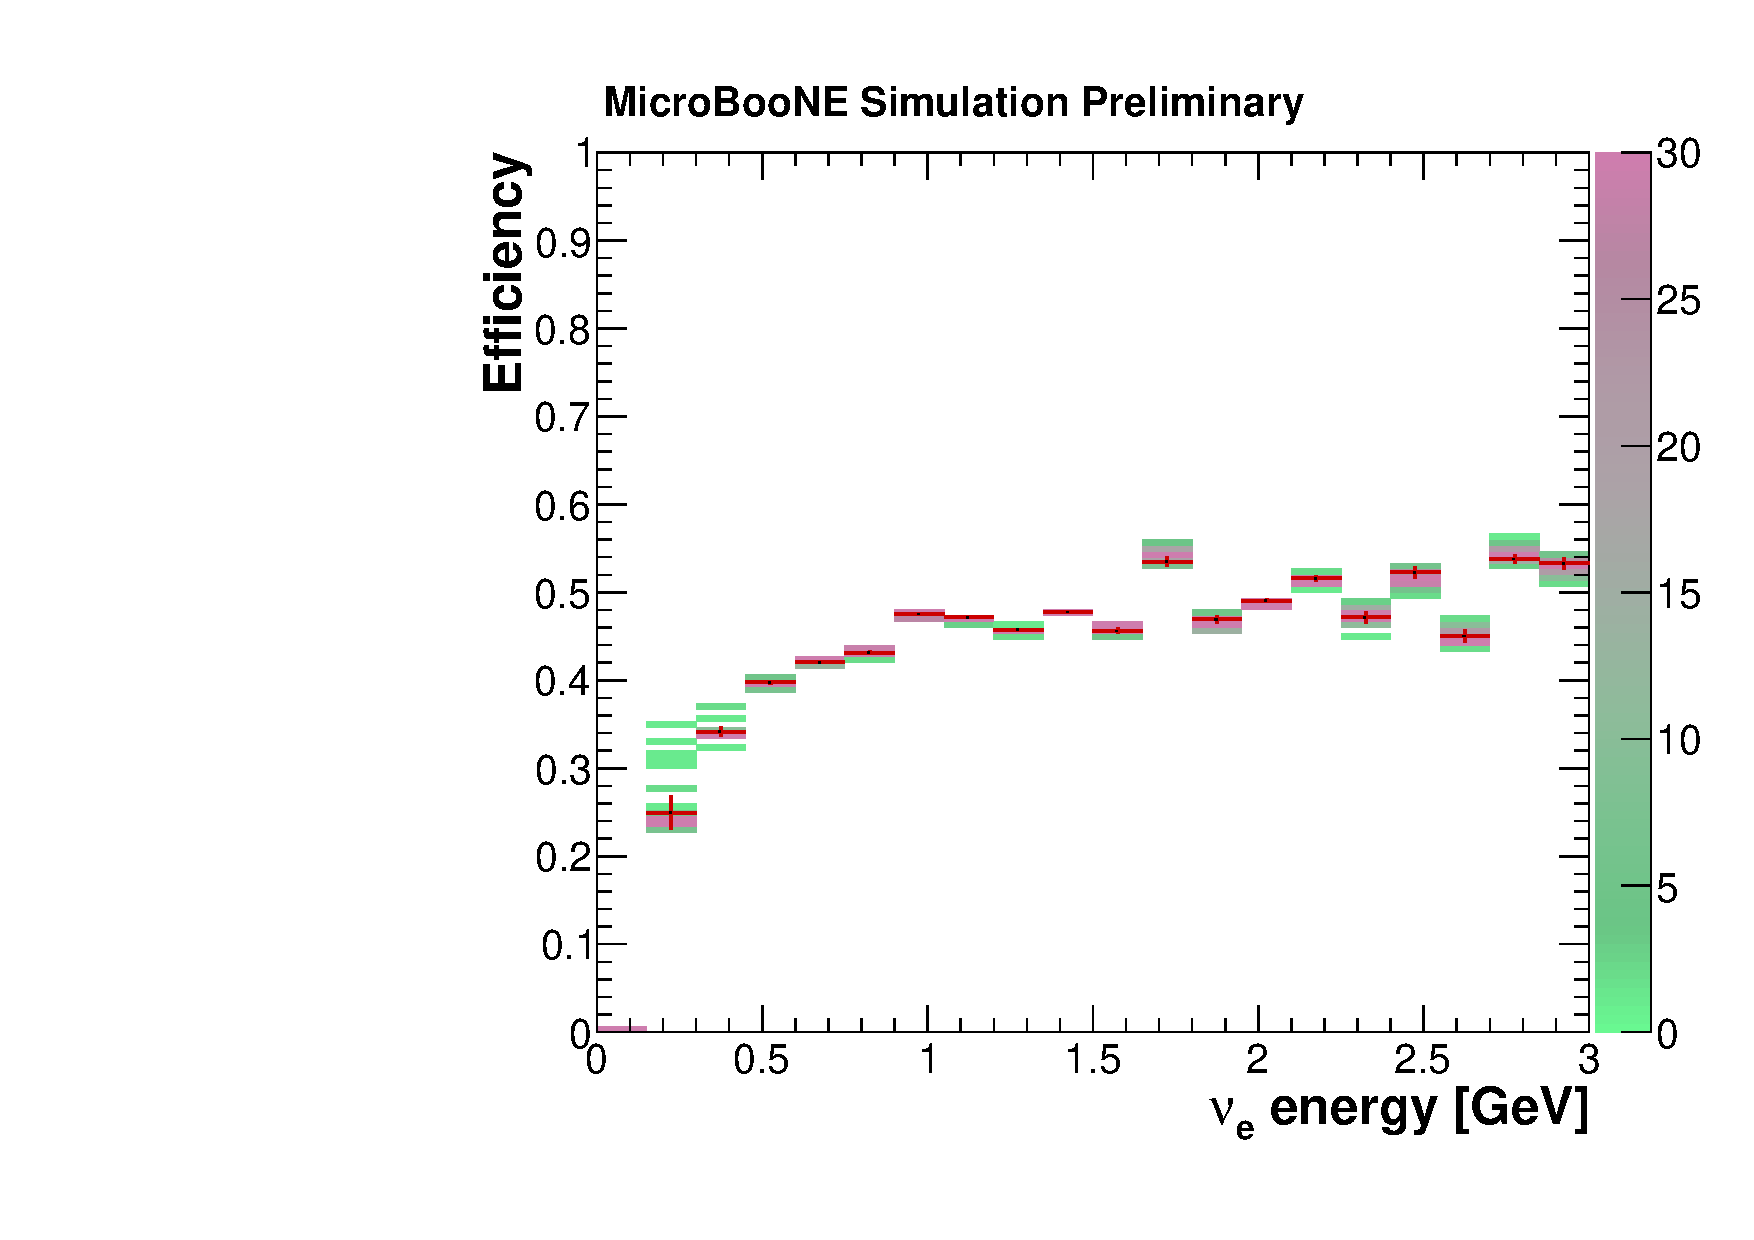
\includegraphics[width=\linewidth]{figures/eff_ene_flux.pdf}
      \caption{$\nu_{e}$ CC0$\pi$-Np selection efficiency.}  \label{fig:eff_flux}
    \end{subfigure}
    \begin{subfigure}{0.45\textwidth}
      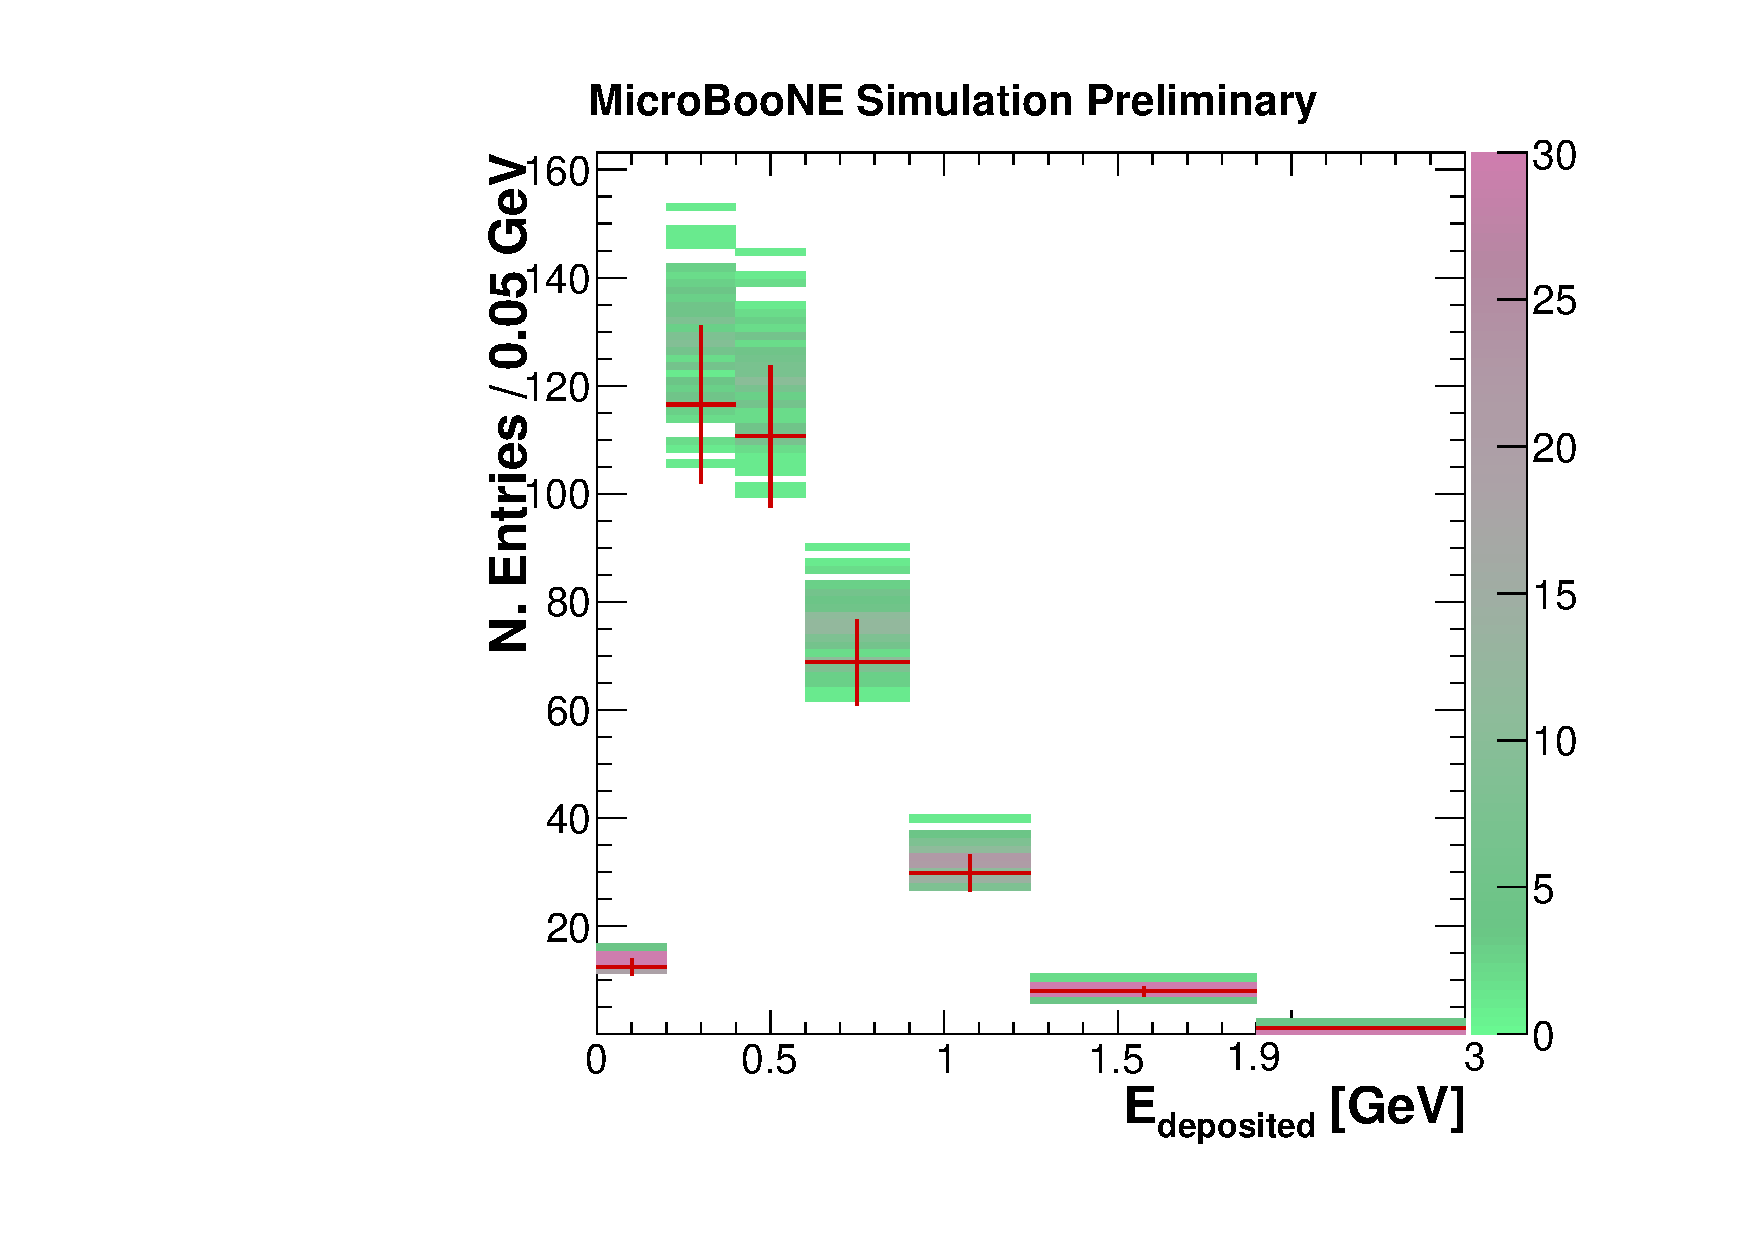
\includegraphics[width=\linewidth]{figures/reco_flux.pdf}
      \caption{$\nu_{e}$ CC0$\pi$-Np candidates energy spectrum in the BNB+cosmic sample.}  \label{fig:reco_flux}
    \end{subfigure}
    \begin{subfigure}{0.45\textwidth}
      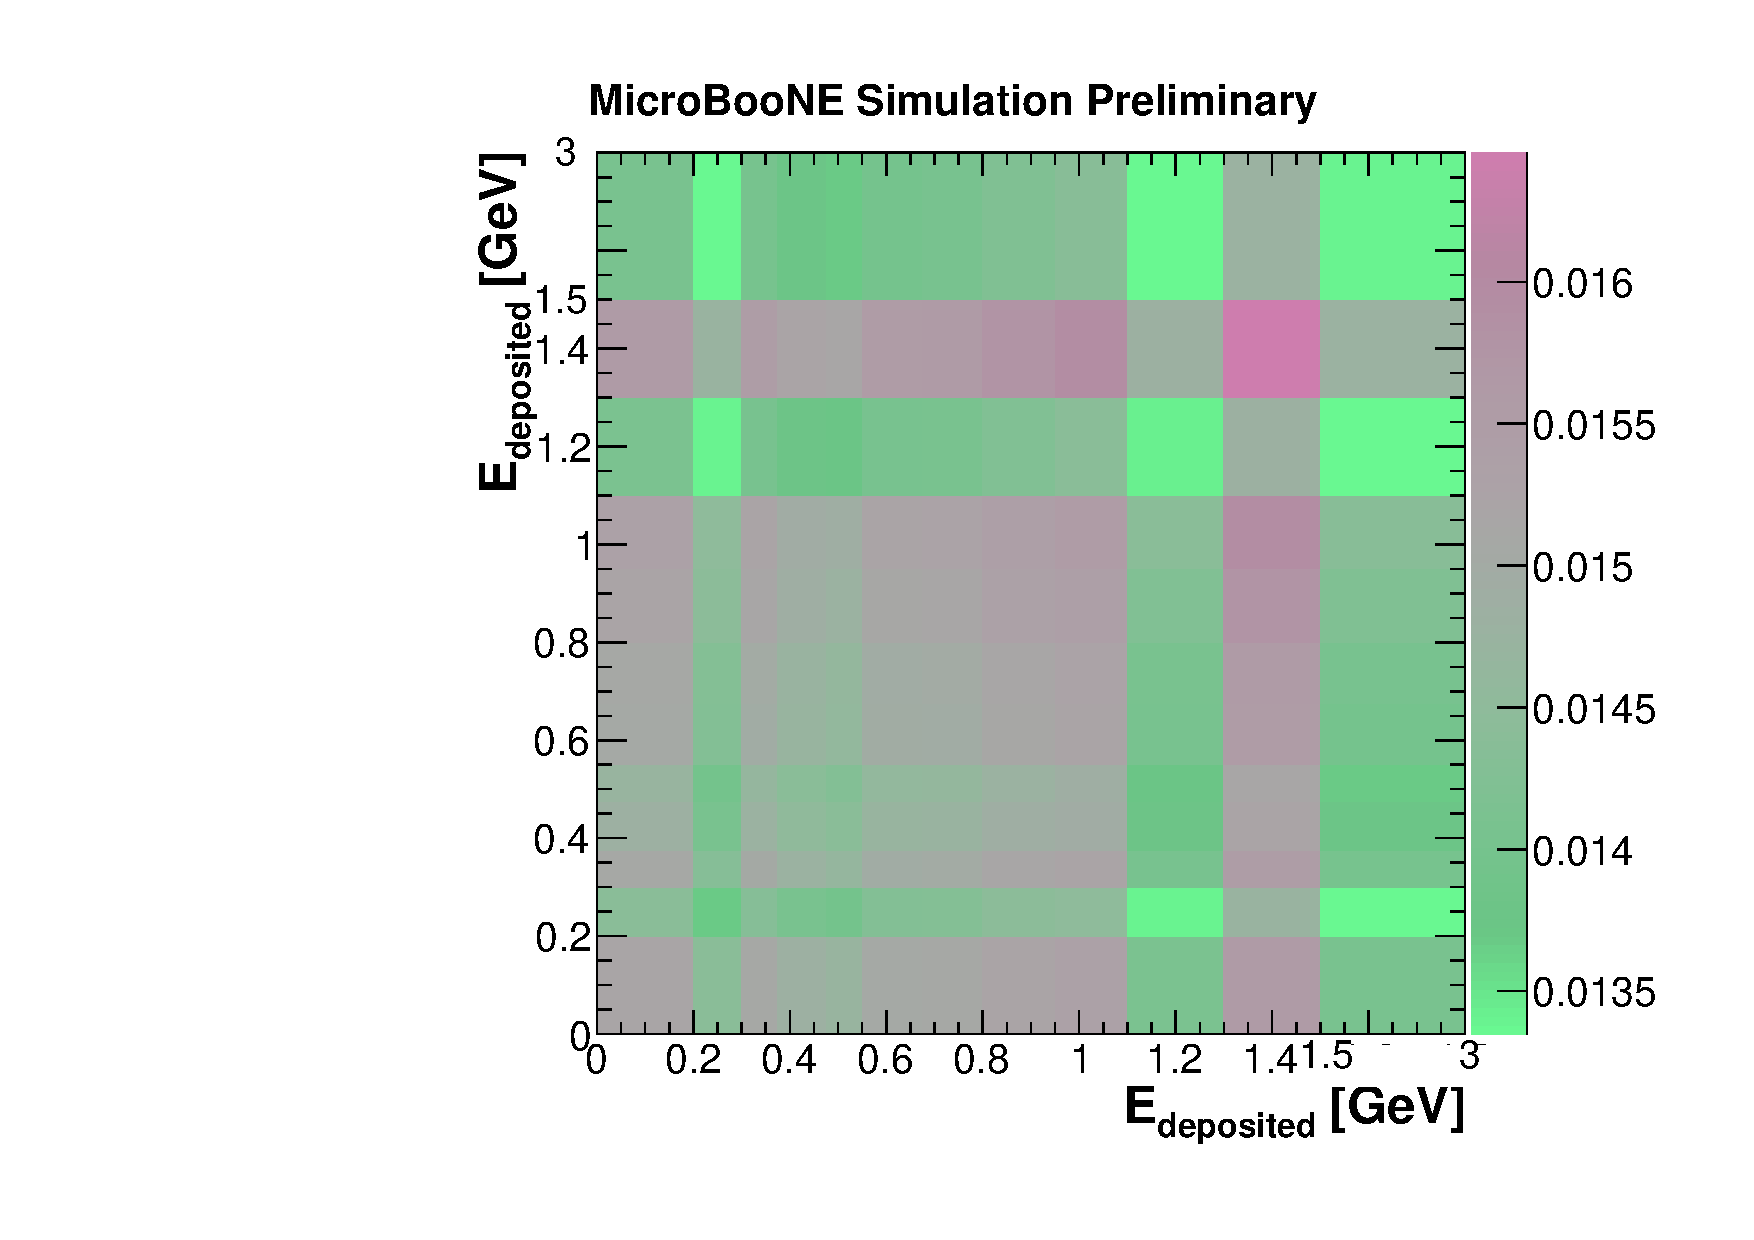
\includegraphics[width=\linewidth]{figures/frac_flux.pdf}
      \caption{Flux variations fractional covariance matrix.}  \label{fig:frac_flux}
    \end{subfigure}
    	\caption{Selection efficiency, reconstructed energy spectrum, and fractional covariance matrix obtained by varying the BNB flux parameters in 100 simulated universes.  The red bars correspond to the central value and its flux systematic uncertainty only.} \label{fig:flux_sys}
	\end{center}
\end{figure}

\subsection{Detector systematic uncertainties}
The detector systematic uncertainties have been measured by simulating several samples where a single detector parameter is varied by its uncertainty or a different physics model is used. In this case, the covariance matrix is evaluated using the definition in eq. \eqref{eq:cov_det}. The fractional covariance matrix and the reconstructed energy spectrum are shown in Figure \ref{fig:frac_det} and Figure \ref{fig:reco_det}, respectively.
The uncertainty related to the detector systematic effects in the number of selected events from the BNB+cosmic sample is 21.9\%. Given the limited size of the detector variation samples, a flat 21.9\% uncertainty is applied to the BNB+cosmic component of the $\nu_{\mu}$ and NC-enhanced samples.

\begin{figure}[htbp]
  \begin{center}
    \begin{subfigure}{0.45\textwidth}
      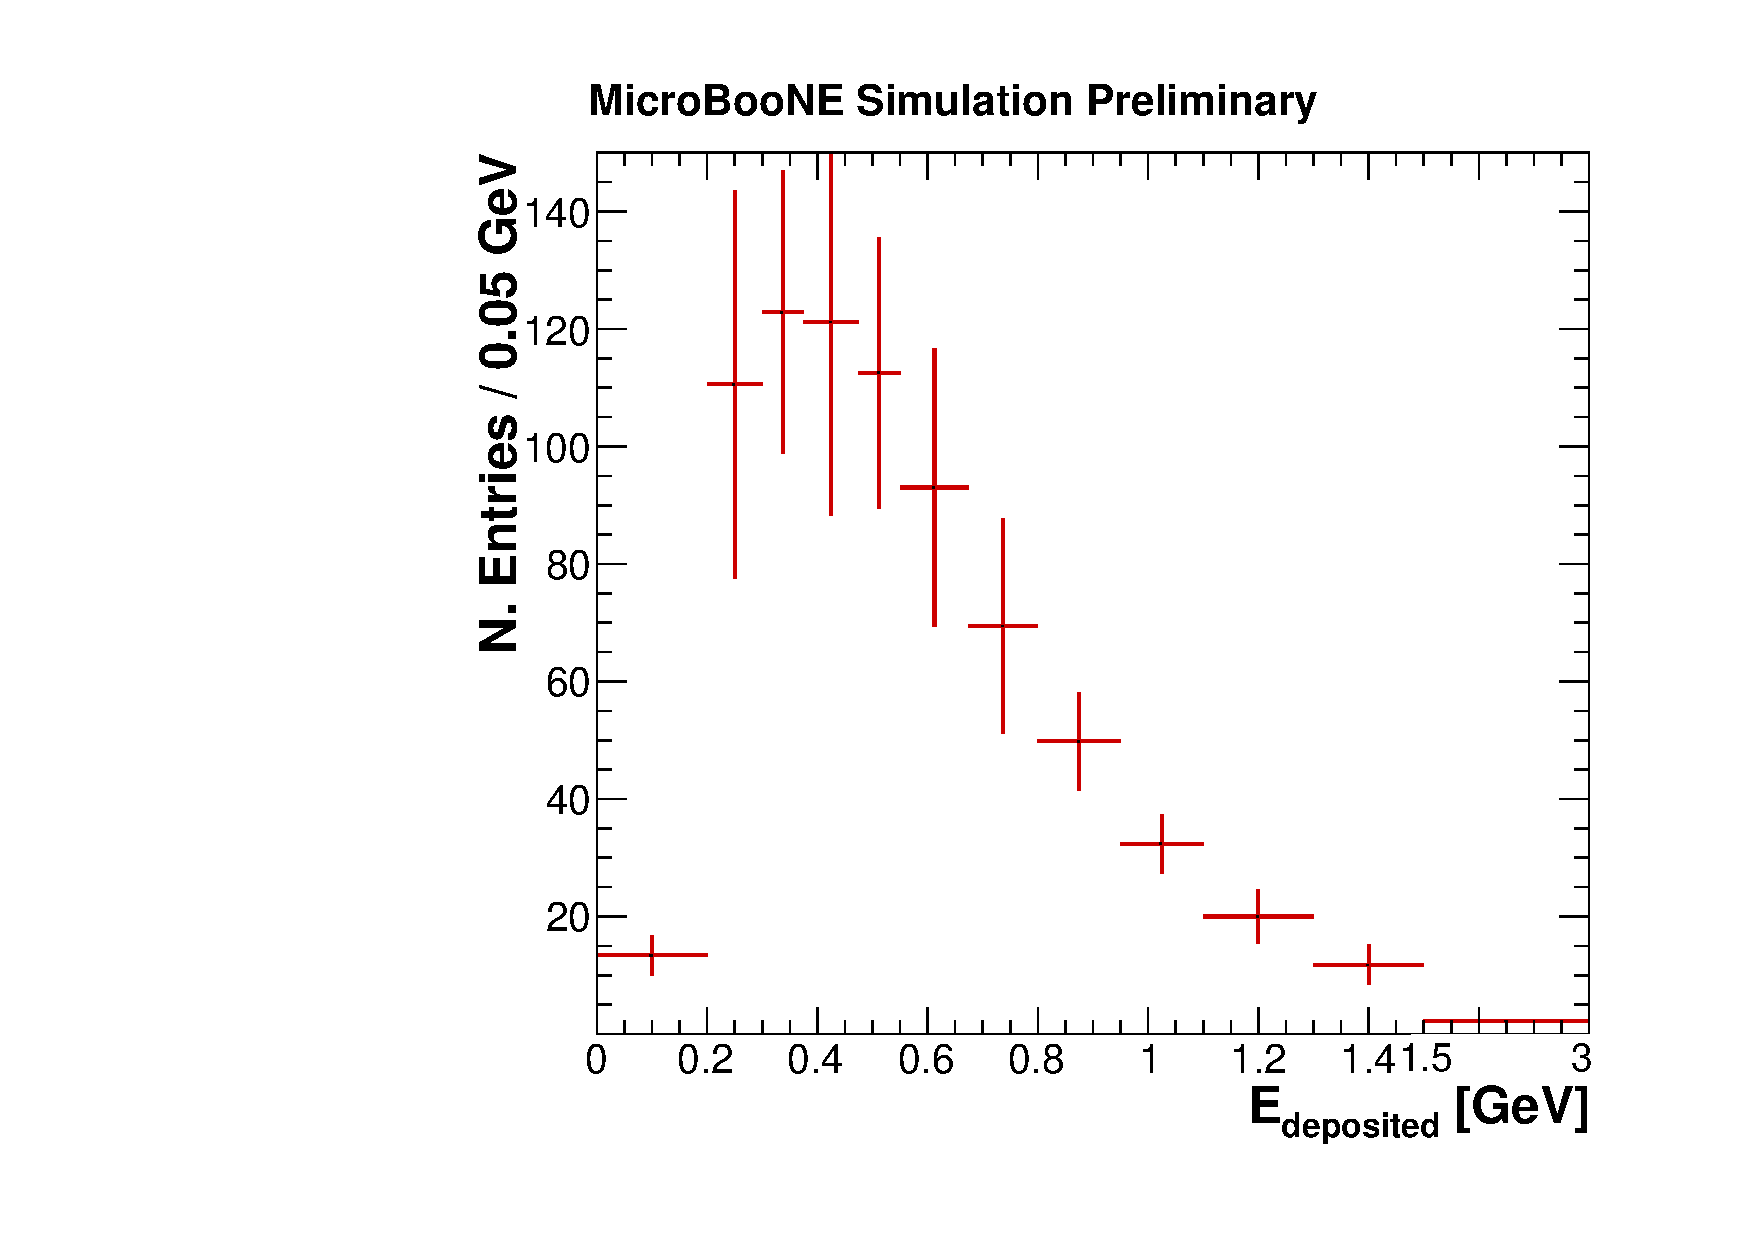
\includegraphics[width=\linewidth]{figures/reco_det.pdf}
      \caption{$\nu_{e}$ CC0$\pi$-Np candidates energy spectrum in the BNB+cosmic sample.}  \label{fig:reco_det}
    \end{subfigure}
    \begin{subfigure}{0.45\textwidth}
      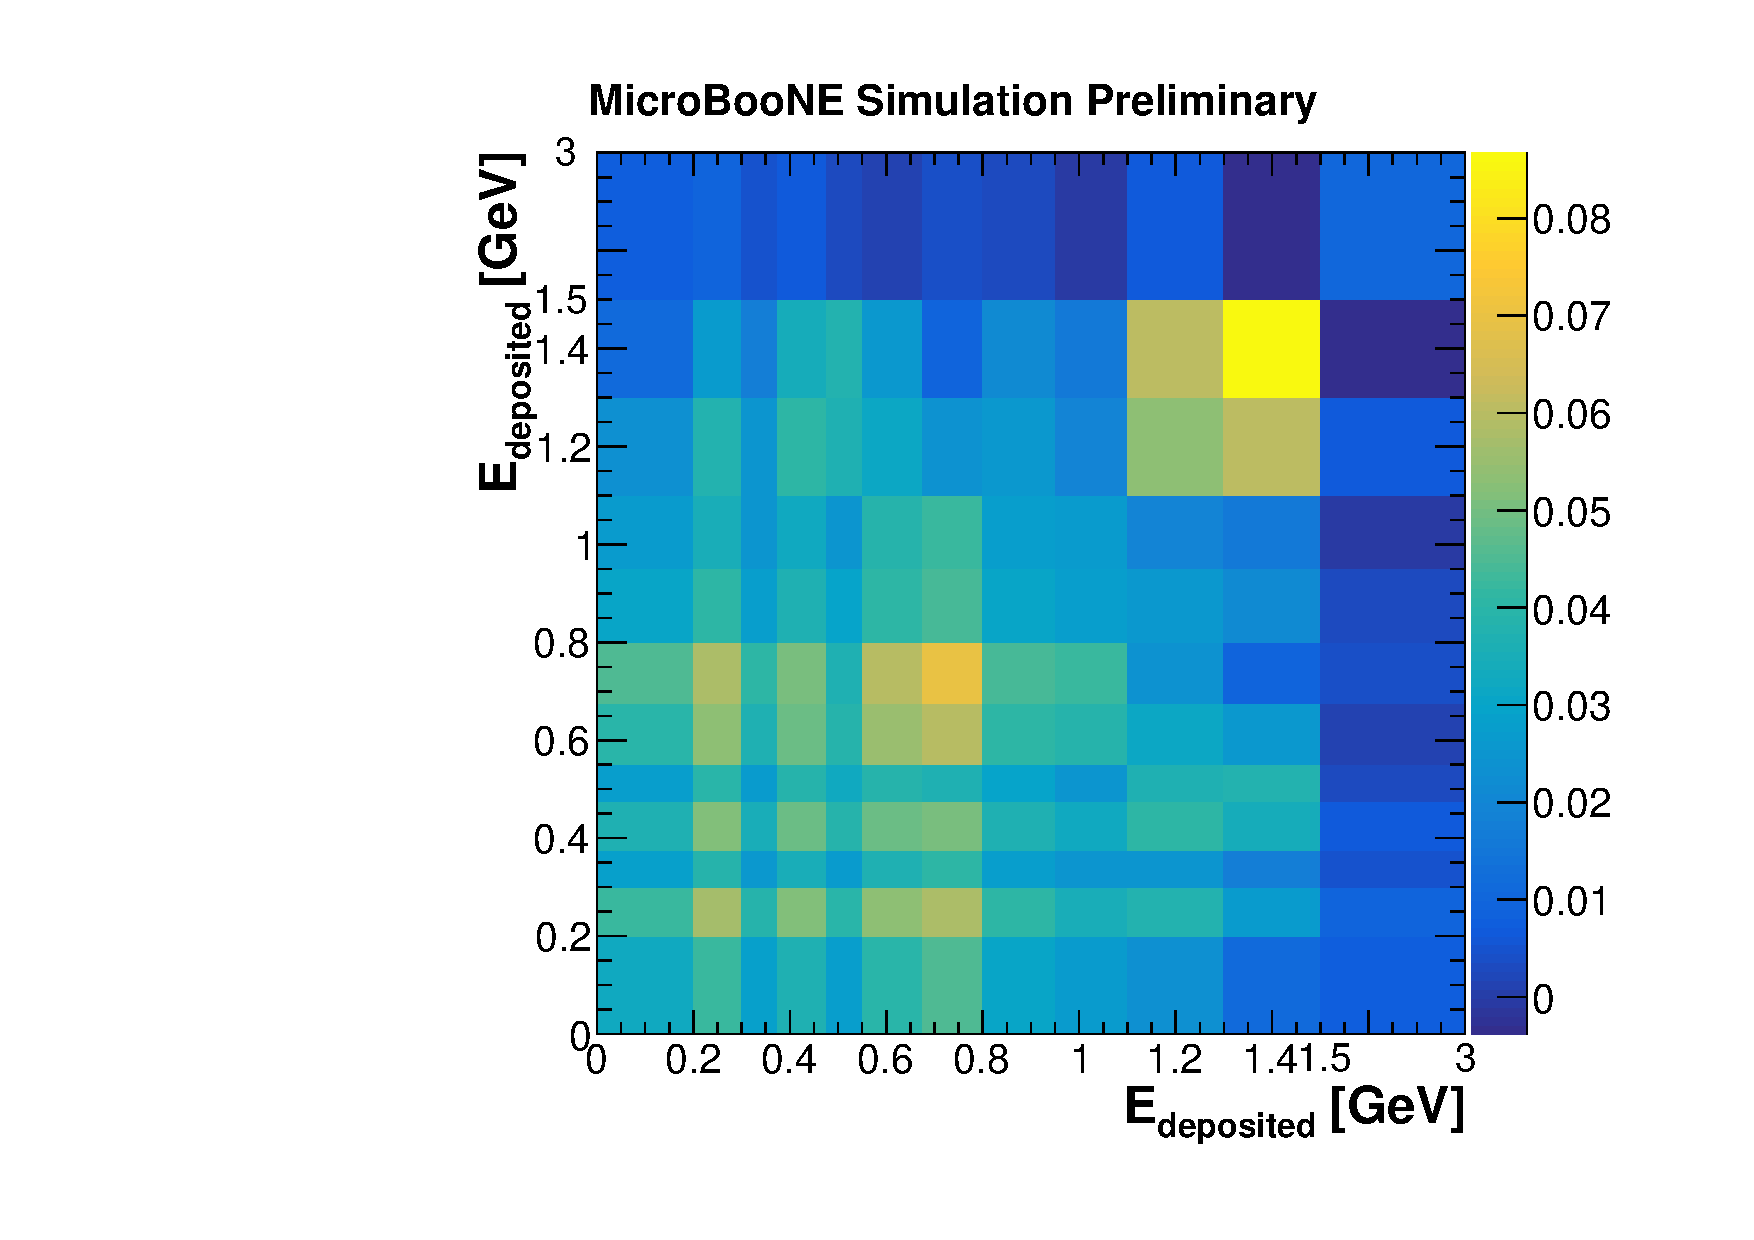
\includegraphics[width=\linewidth]{figures/frac_det.pdf}
      \caption{Detector variations fractional covariance matrix.}  \label{fig:frac_det}
    \end{subfigure}
    	\caption{Reconstructed energy spectrum, and fractional covariance matrix obtained with the detector variations samples.  The red bars correspond to the central value and its detector systematic uncertainty only.} \label{fig:det_sys}
	\end{center}
\end{figure}


\vspace{1em}
Table \ref{tab:syst} shows the uncertainty in the number of selected events from in the BNB+cosmic sample for the GENIE, flux, and detector systematic variations. The total uncertainty, obtained with eq. \ref{eq:cov_tot}, is 21.9~\%. In the POT-normalized figures of Section \ref{sec:methodology}, the uncertainty on the dirt and the $\nu_{e}$ CC$0\pi$-Np samples is assumed to be the same one of the BNB+cosmic sample. Given the small contribution of these samples to the number of selected events (2.5\% of the total), this approximation is considered good enough at this stage. The statistical uncertainty of the data off-beam sample is 1.0\%. 

\begin{table}[htbp]
   \centering
   \begin{tabular}{p{0.23\linewidth}p{0.33\linewidth}p{0.21\linewidth}p{0.11\linewidth}}
     \toprule
     Type & Description & Method & Uncertainty \\
     \midrule
     Monte Carlo statistics & Finite size of the Monte Carlo sample. & - & 1.9~\%\\
     GENIE & Variations of the neutrino generator parameters within their uncertainties. & 100 universes & 7.6~\%\\
     Flux & Variations of the flux simulation parameters within their uncertainties. & 100 universes & 7.8~\%\\
     Space-charge effect & Data-driven estimation of the space-charge effect. & Alternate simulation & 9.7~\%\\
     Dynamic Induced Charge & Improved simulation of the induction of charge on the wires. & Alternate simulation & 9.5~\%\\
     Light simulation & Improved simulation of the light production in the detector. & Alternate simulation & 4.0~\%\\
     Saturated channels & Channels that tends to saturate are turned off in the simulation. & Alternate simulation & 4.2~\%\\
     Misconfigured channels & Channels with misconfigured ASIC gains and shaping are turned off in the simulation. & Alternate simulation & 4.1~\%\\
     Electron lifetime & Lifetime of the electron in the detector is reduced to 10~ms. & Alternate model & 3.9~\%\\
     Recombination model & The Birks model of recombination \cite{birks} is used instead of the modified box model \cite{boxmodel}. & Alternate model & 4.0~\%\\
     Longitudinal diffusion & The longitude diffusion is varied within the uncertainty. & $\pm1\sigma$ variation & 4.5~\%\\
     Transverse diffusion & The transverse diffusion is varied within the uncertainty. & $\pm1\sigma$ variation & 4.8~\%\\
     Wire noise & The amount of noise on the wires is varied within the uncertainty. & $\pm1\sigma$ variation & 3.7~\%\\
     PE noise & The amount of single-PE noise in the PMTs is varied within the uncertainty. & $\pm1\sigma$ variation & 4.8~\%\\
     Cryostat light & The light outside the TPC but inside the cryostat is increased by 50\% & Alternate simulation & 3.8~\%\\
     \midrule
     Total & & & 21.9~\%\\
     \bottomrule
   \end{tabular}
   \caption{Summary of the systematic uncertainties in the number of selected events in the BNB+cosmic sample.}\label{tab:syst}
\end{table}
